\documentclass[10pt]{article}
\usepackage[polish]{babel}
\usepackage[utf8]{inputenc}
\usepackage[T1]{fontenc}
\usepackage{amsmath}
\usepackage{amsfonts}
\usepackage{amssymb}
\usepackage[version=4]{mhchem}
\usepackage{stmaryrd}
\usepackage{graphicx}
\usepackage[export]{adjustbox}
\graphicspath{ {./images/} }
\usepackage{bbold}

%New command to display footnote whose markers will always be hidden
\let\svthefootnote\thefootnote
\newcommand\blfootnotetext[1]{%
  \let\thefootnote\relax\footnote{#1}%
  \addtocounter{footnote}{-1}%
  \let\thefootnote\svthefootnote%
}

%Overriding the \footnotetext command to hide the marker if its value is `0`
\let\svfootnotetext\footnotetext
\renewcommand\footnotetext[2][?]{%
  \if\relax#1\relax%
    \ifnum\value{footnote}=0\blfootnotetext{#2}\else\svfootnotetext{#2}\fi%
  \else%
    \if?#1\ifnum\value{footnote}=0\blfootnotetext{#2}\else\svfootnotetext{#2}\fi%
    \else\svfootnotetext[#1]{#2}\fi%
  \fi
}

\begin{document}
\section*{CENTRALNA \\
 KOMISJA \\
 EGZAMINACYJNA}
\begin{center}
\begin{tabular}{|l|l|}
\hline
Rodzaj dokumentu: & \begin{tabular}{l}
Zasady Oceniania rozwiązań \\
zadań \\
\end{tabular} \\
\hline
Egzamin: & Egzamin maturalny \\
\hline
Przedmiot: & Matematyka \\
\hline
Poziom: & \begin{tabular}{l}
EMAP-P0-100 (wersje arkusza: A i B), \\
EMAP-P0-200, EMAP-P0-300, \\
Formy arkusza: \\
\hline
EMAP-P0-400, EMAP-P0-600, \\
EMAP-P0-700, EMAP-P0-Q00, \\
\hline
Eermin egzaminu: \\
\hline
\end{tabular} \\
\hline
\begin{tabular}{l}
Eata publikacji \\
(okumentu: \\
\end{tabular} & \begin{tabular}{l}
EMAP-P0-Z00, EMAU-P0-100 \\
\hline
\end{tabular} \\
\hline
\end{tabular}
\end{center}

\section*{Uwaga:}
Gdy wymaganie egzaminacyjne dotyczy treści z III etapu edukacyjnego, dopisano „G".

\section*{ZADANIA ZAMKNIETE}
Zadanie 1. (0-1)

\begin{center}
\begin{tabular}{|l|l|}
\hline
\multicolumn{2}{|c|}{Wymagania egzaminacyjne 2023 i 2024 $^{1}$} \\
\hline
\multicolumn{1}{|c|}{Wymaganie ogólne} & \multicolumn{1}{c|}{Wymaganie szczegółowe $^{|c|}$} \\
\hline
\begin{tabular}{l}
II. Wykorzystanie i interpretowanie \\
reprezentacji. \\
\end{tabular} & \begin{tabular}{l}
Zdający: \\
1.6) wykorzystuje definicję logarytmu [...]. \\
\end{tabular} \\
\hline
\end{tabular}
\end{center}

\section*{Zasady oceniania}
1 pkt - odpowiedź poprawna.\\
0 pkt - odpowiedź niepoprawna albo brak odpowiedzi.

\section*{Rozwiązanie}
Wersja A Wersja B\\
D\\
D

\section*{Zadanie 2. (0-1)}
\begin{center}
\begin{tabular}{|l|l|}
\hline
\multicolumn{2}{|c|}{Wymagania egzaminacyjne 2023 i 2024} \\
\hline
\multicolumn{1}{|c|}{Wymaganie ogólne} & \multicolumn{1}{c|}{Wymaganie szczegółowe} \\
\hline
\begin{tabular}{l}
II. Wykorzystanie i interpretowanie \\
reprezentacji. \\
\end{tabular} & \begin{tabular}{l}
Zdajacy: \\
1.3) posługuje się w obliczeniach \\
pierwiastkami dowolnego stopnia i stosuje \\
prawa działań na pierwiastkach. \\
\end{tabular} \\
\hline
\end{tabular}
\end{center}

\section*{Zasady oceniania}
1 pkt - odpowiedź poprawna.\\
0 pkt - odpowiedź niepoprawna albo brak odpowiedzi.

\section*{Rozwiązanie}
Wersja A\\
Wersja B\\
A\\
C

\footnotetext{${ }^{1}$ Rozporządzenie Ministra Edukacji i Nauki z dnia 1 sierpnia 2022 r. w sprawie wymagań egzaminacyjnych dla egzaminu maturalnego przeprowadzanego w roku szkolnym 2022/2023 i 2023/2024 (Dz.U. 2022, poz.1698).
}\section*{Zadanie 3. (0-1)}
\begin{center}
\begin{tabular}{|l|l|}
\hline
\multicolumn{2}{|c|}{Wymagania egzaminacyjne 2023 i 2024} \\
\hline
\multicolumn{1}{|c|}{Wymaganie ogólne} & \multicolumn{1}{c|}{Wymaganie szczegółowe} \\
\hline
I. Wykorzystanie i tworzenie informacji. & \begin{tabular}{l}
Zdający: \\
 \\
 \\
\hline
\end{tabular} 1.8) wykonuje obliczenia procentowe [...]. \\
\hline
\end{tabular}
\end{center}

\section*{Zasady oceniania}
1 pkt - odpowiedź poprawna.\\
0 pkt - odpowiedź niepoprawna albo brak odpowiedzi.

\section*{Rozwiązanie}
Wersja A\\
A

Wersja B\\
A

\section*{Zadanie 4. (0-1)}
\begin{center}
\begin{tabular}{|l|l|}
\hline
\multicolumn{2}{|c|}{Wymagania egzaminacyjne 2023 i 2024} \\
\hline
\multicolumn{1}{|c|}{Wymaganie ogólne} & \multicolumn{1}{c|}{Wymaganie szczegółowe} \\
\hline
II. Wykorzystanie i interpretowanie & Zdajacy: \\
reprezentacji. & \begin{tabular}{l}
2. używa wzorów skróconego mnożenia na \\
 \\
\end{tabular}$(a \pm b)^{2}$ oraz $a^{2}-b^{2}$. \\
\hline
\end{tabular}
\end{center}

\section*{Zasady oceniania}
1 pkt - odpowiedź poprawna.\\
0 pkt - odpowiedź niepoprawna albo brak odpowiedzi.

\section*{Rozwiązanie}
Wersja A\\
Wersja B\\
A\\
B

\section*{Zadanie 5. (0-1)}
\begin{center}
\begin{tabular}{|l|l|}
\hline
\multicolumn{2}{|c|}{Wymagania egzaminacyjne 2023 i 2024} \\
\hline
\multicolumn{1}{|c|}{Wymaganie ogólne} & \multicolumn{1}{c|}{Wymaganie szczegółowe} \\
\hline
II. Wykorzystanie i interpretowanie & \begin{tabular}{l}
Zdajacy: \\
reprezentacji. \\
\end{tabular} \\
 & \begin{tabular}{l}
3.2) wykorzystuje interpretacje \\
geometryczną układu równań stopnia \\
pierwszego z dwiema niewiadomymi. \\
\end{tabular} \\
\hline
\end{tabular}
\end{center}

\section*{Zasady oceniania}
1 pkt - odpowiedź poprawna.\\
0 pkt - odpowiedź niepoprawna albo brak odpowiedzi.

\section*{Rozwiązanie}
Wersja A\\
D

Wersja B\\
A

\section*{Zadanie 6. (0-1)}
\begin{center}
\begin{tabular}{|l|l|}
\hline
\multicolumn{2}{|c|}{Wymagania egzaminacyjne 2023 i 2024} \\
\hline
\multicolumn{1}{|c|}{Wymaganie ogólne} & \multicolumn{1}{c|}{Wymaganie szczegółowe} \\
\hline
\begin{tabular}{ll}
\multicolumn{1}{|c|}{II. Wykorzystanie i interpretowanie} & \begin{tabular}{l}
Zdający: \\
reprezentacji. \\
\end{tabular} \\
\hline
\end{tabular}\begin{tabular}{l}
3.3) rozwiązuje nierówności stopnia \\
pierwszego z jedną niewiadomą. \\
\end{tabular} &  \\
\hline
\end{tabular}
\end{center}

\section*{Zasady oceniania}
1 pkt - odpowiedź poprawna.\\
0 pkt - odpowiedź niepoprawna albo brak odpowiedzi.

\section*{Rozwiązanie}
$\begin{array}{ll}\text { Wersja A } & \text { Wersja B } \\ \text { C } & \text { A }\end{array}$

Zadanie 7. (0-1)

\begin{center}
\begin{tabular}{|l|l|}
\hline
\multicolumn{2}{|c|}{Wymagania egzaminacyjne 2023 i 2024} \\
\hline
\multicolumn{1}{|c|}{Wymaganie ogólne} & \multicolumn{1}{c|}{Wymaganie szczegółowe} \\
\hline
II. Wykorzystanie i interpretowanie & Zdający: \\
reprezentacji. & 3.6) korzysta z własności iloczynu przy \\
 & rozwiązywaniu równań typu \\
 & $x(x+1)(x-7)=0$. \\
\hline
\end{tabular}
\end{center}

\section*{Zasady oceniania}
1 pkt - odpowiedź poprawna.\\
0 pkt - odpowiedź niepoprawna albo brak odpowiedzi.

\section*{Rozwiązanie}
Wersja A\\
D

Wersja B\\
C

\section*{Zadanie 8. (0-1)}
\begin{center}
\begin{tabular}{|l|l|}
\hline
\multicolumn{2}{|c|}{Wymagania egzaminacyjne 2023 i 2024} \\
\hline
\multicolumn{1}{|c|}{Wymaganie ogólne} & \multicolumn{1}{c|}{Wymaganie szczegółowe} \\
\hline
\multicolumn{1}{|c|}{II. Wykorzystanie i interpretowanie} & \begin{tabular}{l}
Zdający: \\
reprezentacji. \\
\end{tabular} \\
\begin{tabular}{l}
3.7) rozwiązuje proste równania wymierne, \\
prowadzące do równań liniowych lub \\
kwadratowych [...]. \\
\end{tabular} &  \\
\hline
\end{tabular}
\end{center}

\section*{Zasady oceniania}
1 pkt - odpowiedź poprawna.\\
0 pkt - odpowiedź niepoprawna albo brak odpowiedzi.

\section*{Rozwiązanie}
Wersja A\\
A

Wersja B\\
A

\section*{Zadanie 9. (0-1)}
\begin{center}
\begin{tabular}{|l|l|}
\hline
\multicolumn{2}{|c|}{Wymagania egzaminacyjne 2023 i 2024} \\
\hline
\multicolumn{1}{|c|}{Wymaganie ogólne} & \multicolumn{1}{c|}{Wymaganie szczegółowe} \\
\hline
I. Wykorzystanie i tworzenie informacji. & \begin{tabular}{l}
Zdający: \\
 \\
 \\
 \\
 \\
 \\
 \\
 \\
 \\
 \\
\hline
\end{tabular}\begin{tabular}{l}
rozwiązywania równán do obliczenia, dla \\
jakiego argumentu funkcja przyjmuje daną \\
wartość. \\
\end{tabular} \\
\hline
\end{tabular}
\end{center}

\section*{Zasady oceniania}
1 pkt - odpowiedź poprawna.\\
0 pkt - odpowiedź niepoprawna albo brak odpowiedzi.

\section*{Rozwiązanie}
\section*{Wersja A}
\section*{B}
Wersja B\\
D

\section*{Zadanie 10. (0-1)}
\begin{center}
\begin{tabular}{|l|l|}
\hline
\multicolumn{2}{|c|}{Wymagania egzaminacyjne 2023 i 2024} \\
\hline
\multicolumn{1}{|c|}{Wymaganie ogólne} & \multicolumn{1}{c|}{Wymaganie szczegółowe} \\
\hline
\begin{tabular}{l}
II. Wykorzystanie i interpretowanie \\
reprezentacji. \\
\end{tabular} & \begin{tabular}{l}
Zdający: \\
 \\
\hline
\end{tabular} \\
\hline
\end{tabular}
\end{center}

\section*{Zasady oceniania}
1 pkt - odpowiedź poprawna.\\
0 pkt - odpowiedź niepoprawna albo brak odpowiedzi.

\section*{Rozwiązanie}
Wersja A\\
C

Wersja B\\
A

Zadanie 11. (0-1)

\begin{center}
\begin{tabular}{|l|l|}
\hline
\multicolumn{2}{|c|}{Wymagania egzaminacyjne 2023 i 2024} \\
\hline
\multicolumn{1}{|c|}{Wymaganie ogólne} & \multicolumn{1}{c|}{Wymaganie szczegółowe} \\
\hline
I. Wykorzystanie i tworzenie informacji. & \begin{tabular}{l}
Zdający: \\
 \\
 \\
 \\
 \\
\hline
\end{tabular}\begin{tabular}{l}
4.3) odczytuje z wykresu własności funkcji \\
(dziedzinę [...]). \\
\end{tabular} \\
\hline
\end{tabular}
\end{center}

\section*{Zasady oceniania}
1 pkt - odpowiedź poprawna.\\
0 pkt - odpowiedź niepoprawna albo brak odpowiedzi.

\section*{Rozwiązanie}
Wersja A Wersja B\\
A\\
C

Zadanie 12. (0-1)

\begin{center}
\begin{tabular}{|l|l|}
\hline
\multicolumn{2}{|c|}{Wymagania egzaminacyjne 2023 i 2024} \\
\hline
\multicolumn{1}{|c|}{Wymaganie ogólne} & \multicolumn{1}{c|}{Wymaganie szczegółowe} \\
\hline
I. Wykorzystanie i tworzenie informacji. & Zdajacy: \\
 & 4.3) odczytuje z wykresu własności funkcji \\
 & ([...] maksymalne przedziały, w których \\
funkcja maleje [...]). &  \\
\hline
\end{tabular}
\end{center}

\section*{Zasady oceniania}
1 pkt - odpowiedź poprawna.\\
0 pkt - odpowiedź niepoprawna albo brak odpowiedzi.

\section*{Rozwiązanie}
Wersja A\\
Wersja B\\
D\\
C

Zadanie 13. (0-1)

\begin{center}
\begin{tabular}{|l|l|}
\hline
\multicolumn{2}{|c|}{Wymagania egzaminacyjne 2023 i 2024} \\
\hline
\multicolumn{1}{|c|}{Wymaganie ogólne} & \multicolumn{1}{c|}{Wymaganie szczegółowe} \\
\hline
I. Wykorzystanie i tworzenie informacji. & \begin{tabular}{l}
Zdający: \\
 \\
 \\
 \\
 \\
\hline
\end{tabular} 4.3) odczytuje z wykresu własności funkcji \\
([...] wartość największą [...]). &  \\
\hline
\end{tabular}
\end{center}

\section*{Zasady oceniania}
1 pkt - odpowiedź poprawna.\\
0 pkt - odpowiedź niepoprawna albo brak odpowiedzi.

\section*{Rozwiązanie}
Wersja A Wersja B\\
C B

Zadanie 14. (0-1)

\begin{center}
\begin{tabular}{|l|l|}
\hline
\multicolumn{2}{|c|}{Wymagania egzaminacyjne 2023 i 2024} \\
\hline
\multicolumn{1}{|c|}{Wymaganie ogólne} & \multicolumn{1}{c|}{Wymaganie szczegółowe} \\
\hline
I. Wykorzystanie i tworzenie informacji. & \begin{tabular}{l}
Zdajacy: \\
 \\
 \\
 \\
 \\
 \\
 \\
 \\
\hline
\end{tabular} kwadratowej do interpretacji zagadnień \\
geometrycznych [...]. &  \\
\hline
\end{tabular}
\end{center}

\section*{Zasady oceniania}
1 pkt - odpowiedź poprawna.\\
0 pkt - odpowiedź niepoprawna albo brak odpowiedzi.

\section*{Rozwiązanie}
Wersja A\\
Wersja B\\
A\\
C

Zadanie 15. (0-1)

\begin{center}
\begin{tabular}{|l|l|}
\hline
\multicolumn{2}{|c|}{Wymagania egzaminacyjne 2023 i 2024} \\
\hline
\multicolumn{1}{|c|}{Wymaganie ogólne} & \multicolumn{1}{c|}{Wymaganie szczegółowe} \\
\hline
\begin{tabular}{ll}
\multicolumn{1}{|c|}{II. Wykorzystanie i interpretowanie} & Zdajacy: \\
reprezentacji. & 5.1) wyznacza wyrazy ciągu określonego \\
 & wzorem ogólnym. \\
\hline
\end{tabular} &  \\
\hline
\end{tabular}
\end{center}

\section*{Zasady oceniania}
1 pkt - odpowiedź poprawna.\\
0 pkt - odpowiedź niepoprawna albo brak odpowiedzi.

\section*{Rozwiązanie}
Wersja A\\
D

Wersja B\\
A

Zadanie 16. (0-1)

\begin{center}
\begin{tabular}{|l|l|}
\hline
\multicolumn{2}{|c|}{Wymagania egzaminacyjne 2023 i 2024} \\
\hline
\multicolumn{1}{|c|}{Wymaganie ogólne} & \multicolumn{1}{|c|}{Wymaganie szczegółowe} \\
\hline
III. Modelowanie matematyczne. & \begin{tabular}{l}
Zdający: \\
$5.4)$ stosuje wzór na $n$-ty wyraz [...] ciągu \\
geometrycznego. \\
\end{tabular} \\
\hline
\end{tabular}
\end{center}

\section*{Zasady oceniania}
1 pkt - odpowiedź poprawna.\\
0 pkt - odpowiedź niepoprawna albo brak odpowiedzi.

\section*{Rozwiązanie}
Wersja A\\
C

Wersja B\\
D

\section*{Zadanie 17. (0-1)}
\begin{center}
\begin{tabular}{|l|l|}
\hline
\multicolumn{2}{|c|}{Wymagania egzaminacyjne 2023 i 2024} \\
\hline
\multicolumn{1}{|c|}{Wymaganie ogólne} & \multicolumn{1}{c|}{Wymaganie szczegółowe} \\
\hline
II. Wykorzystanie i interpretowanie & Zdający: \\
reprezentacji. & \begin{tabular}{l}
6.1) wykorzystuje definicje i wyznacza \\
 \\
 \\
 \\
 \\
 \\
 \\
wartości funkcji $[\ldots]$ tangens kątów \\
o miarach od $0^{\circ}$ do $180^{\circ}$. \\
\hline
\end{tabular} \\
\hline
\end{tabular}
\end{center}

\section*{Zasady oceniania}
1 pkt - odpowiedź poprawna.\\
0 pkt - odpowiedź niepoprawna albo brak odpowiedzi.

\section*{Rozwiązanie}
\section*{Wersja A}
D

Wersja B\\
B

\section*{Zadanie 18. (0-1)}
\begin{center}
\begin{tabular}{|l|l|}
\hline
\multicolumn{2}{|c|}{Wymagania egzaminacyjne 2023 i 2024} \\
\hline
\multicolumn{1}{|c|}{Wymaganie ogólne} & \multicolumn{1}{|c|}{Wymaganie szczegółowe} \\
\hline
IV. Użycie i tworzenie strategii. & \begin{tabular}{l}
Zdający: \\
 \\
 \\
 \\
 \\
 \\
 \\
 \\
 \\
6.3) stosuje proste zależności między \\
funkjami trygonometrycznymi: \\
$\sin ^{2} \alpha+\cos ^{2} \alpha=1 \quad[\ldots]$. \\
\end{tabular} \\
\hline
\end{tabular}
\end{center}

\section*{Zasady oceniania}
1 pkt - odpowiedź poprawna.\\
0 pkt - odpowiedź niepoprawna albo brak odpowiedzi.

\section*{Rozwiązanie}
Wersja A Wersja B\\
A\\
C

Zadanie 19. (0-1)

\begin{center}
\begin{tabular}{|l|l|}
\hline
\multicolumn{2}{|c|}{Wymagania egzaminacyjne 2023 i 2024} \\
\hline
\multicolumn{1}{|c|}{Wymaganie ogólne} & \multicolumn{1}{c|}{Wymaganie szczegółowe} \\
\hline
IV. Użycie i tworzenie strategii. & \begin{tabular}{l}
Zdający: \\
 \\
 \\
 \\
 \\
 \\
\hline
\end{tabular} środkosuje zależności między kątem i kątem wpisanym. \\
\hline
\end{tabular}
\end{center}

\section*{Zasady oceniania}
1 pkt - odpowiedź poprawna.\\
0 pkt - odpowiedź niepoprawna albo brak odpowiedzi.

\section*{Rozwiązanie}
Wersja A\\
Wersja B\\
B\\
C

Zadanie 20. (0-1)

\begin{center}
\begin{tabular}{|l|l|}
\hline
\multicolumn{2}{|c|}{Wymagania egzaminacyjne 2023 i 2024} \\
\hline
\multicolumn{1}{|c|}{Wymaganie ogólne} & \multicolumn{1}{c|}{Wymaganie szczegółowe} \\
\hline
I. Wykorzystanie i tworzenie informacji. & Zdający: \\
 & G10.8) korzysta z własności kątów \\
i przekąnych w [...] rombach [...]. &  \\
\hline
\end{tabular}
\end{center}

\section*{Zasady oceniania}
1 pkt - odpowiedź poprawna.\\
0 pkt - odpowiedź niepoprawna albo brak odpowiedzi.

\section*{Rozwiązanie}
Wersja A\\
Wersja B\\
B\\
D

\section*{Zadanie 21. (0-1)}
\begin{center}
\begin{tabular}{|l|l|}
\hline
\multicolumn{2}{|c|}{Wymagania egzaminacyjne 2023 i 2024} \\
\hline
\multicolumn{1}{|c|}{Wymaganie ogólne} & \multicolumn{1}{c|}{Wymaganie szczegółowe} \\
\hline
\begin{tabular}{ll}
II. Wykorzystanie i interpretowanie \\
reprezentacji. \\
\end{tabular} & \begin{tabular}{l}
Zdający: \\
 \\
\hline
\end{tabular} \\
\hline
\end{tabular}
\end{center}

\section*{Zasady oceniania}
1 pkt - odpowiedź poprawna.\\
0 pkt - odpowiedź niepoprawna albo brak odpowiedzi.

\section*{Rozwiązanie}
Wersja A Wersja B\\
C B

\section*{Zadanie 22. (0-1)}
\begin{center}
\begin{tabular}{|l|l|}
\hline
\multicolumn{2}{|c|}{Wymagania egzaminacyjne 2023 i 2024} \\
\hline
\multicolumn{1}{|c|}{Wymaganie ogólne} & \multicolumn{1}{c|}{Wymaganie szczegółowe} \\
\hline
\begin{tabular}{l}
II. Wykorzystanie i interpretowanie \\
reprezentacji. \\
\end{tabular} & \begin{tabular}{l}
Zdający: \\
7.4) korzysta z własności funkcji \\
trygonometrycznych w łatwych obliczeniach \\
geometrycznych [...]. \\
\end{tabular} \\
\hline
\end{tabular}
\end{center}

\section*{Zasady oceniania}
1 pkt - odpowiedź poprawna.\\
0 pkt - odpowiedź niepoprawna albo brak odpowiedzi.

\section*{Rozwiązanie}
Wersja A\\
Wersja B\\
A\\
B

Zadanie 23. (0-1)

\begin{center}
\begin{tabular}{|l|l|}
\hline
\multicolumn{2}{|c|}{Wymagania egzaminacyjne 2023 i 2024} \\
\hline
\multicolumn{1}{|c|}{Wymaganie ogólne} & \multicolumn{1}{c|}{Wymaganie szczegółowe} \\
\hline
II. Wykorzystanie i interpretowanie & Zdajacy: \\
reprezentacji. & 8.3) wyznacza równanie prostej, która jest \\
 & równoległa [...] do prostej danej w postaci \\
 & kierunkowej i przechodzi przez dany punkt. \\
\hline
\end{tabular}
\end{center}

\section*{Zasady oceniania}
1 pkt - odpowiedź poprawna.\\
0 pkt - odpowiedź niepoprawna albo brak odpowiedzi.

\section*{Rozwiązanie}
$\begin{array}{ll}\text { Wersja A } & \text { Wersja B } \\ \text { D } & \text { B }\end{array}$

\section*{Zadanie 24. (0-1)}
\begin{center}
\begin{tabular}{|l|l|}
\hline
\multicolumn{2}{|c|}{Wymagania egzaminacyjne 2023 i 2024} \\
\hline
\multicolumn{1}{|c|}{Wymaganie ogólne} & \multicolumn{1}{c|}{Wymaganie szczegółowe} \\
\hline
I. Wykorzystanie i tworzenie informacji. & Zdający: \\
 & 8.5) wyznacza współrzędne środka odcinka. \\
\hline
\end{tabular}
\end{center}

\section*{Zasady oceniania}
1 pkt - odpowiedź poprawna.\\
0 pkt - odpowiedź niepoprawna albo brak odpowiedzi.

\section*{Rozwiązanie}
Wersja A\\
B

Wersja B\\
A

Zadanie 25. (0-1)

\begin{center}
\begin{tabular}{|l|l|}
\hline
\multicolumn{2}{|c|}{Wymagania egzaminacyjne 2023 i 2024} \\
\hline
\multicolumn{1}{|c|}{Wymaganie ogólne} & \multicolumn{1}{c|}{Wymaganie szczegółowe} \\
\hline
II. Wykorzystanie i interpretowanie & Zdający: \\
reprezentacji. & 8.7) znajduje obrazy niektórych figur \\
 & geometrycznych ([...] prostej [...]) \\
 & w [...] symetrii środkowej względem \\
 & początku układu. \\
\hline
\end{tabular}
\end{center}

\section*{Zasady oceniania}
1 pkt - odpowiedź poprawna.\\
0 pkt - odpowiedź niepoprawna albo brak odpowiedzi.

\section*{Rozwiązanie}
Wersja A\\
A

Wersja B\\
D

Zadanie 26. (0-1)

\begin{center}
\begin{tabular}{|l|l|}
\hline
\multicolumn{2}{|c|}{Wymagania egzaminacyjne 2023 i 2024} \\
\hline
\multicolumn{1}{|c|}{Wymaganie ogólne} & \multicolumn{1}{c|}{Wymagania szczegółowe} \\
\hline
II. Wykorzystanie i interpretowanie & Zdający: \\
reprezentacji. & 9.1) rozpoznaje w graniastosłupach kąty \\
 & między odcinkami [...]; \\
 & 9.3) stosuje trygonometrię do obliczeń \\
 & długości odcinków [...]. \\
\hline
\end{tabular}
\end{center}

\section*{Zasady oceniania}
1 pkt - odpowiedź poprawna.\\
0 pkt - odpowiedź niepoprawna albo brak odpowiedzi.

\section*{Rozwiązanie}
Wersja A\\
Wersja B\\
B\\
D

Zadanie 27. (0-1)

\begin{center}
\begin{tabular}{|l|l|}
\hline
\multicolumn{2}{|c|}{Wymagania egzaminacyjne 2023 i 2024} \\
\hline
\multicolumn{1}{|c|}{Wymaganie ogólne} & \multicolumn{1}{c|}{Wymaganie szczegółowe} \\
\hline
\begin{tabular}{ll}
\multicolumn{1}{|c|}{II. Wykorzystanie i interpretowanie} & \begin{tabular}{l}
Zdający: \\
reprezentacji. \\
\end{tabular} \\
 & G9.3) wyznacza średnią arytmetyczną [...] \\
zestawu danych. &  \\
\end{tabular} &  \\
\hline
\end{tabular}
\end{center}

\section*{Zasady oceniania}
1 pkt - odpowiedź poprawna.\\
0 pkt - odpowiedź niepoprawna albo brak odpowiedzi.

\section*{Rozwiązanie}
Wersja A\\
Wersja B\\
C\\
B

\section*{Zadanie 28. (0-1)}
\begin{center}
\begin{tabular}{|l|l|}
\hline
\multicolumn{2}{|c|}{Wymagania egzaminacyjne 2023 i 2024} \\
\hline
\multicolumn{1}{|c|}{Wymaganie ogólne} & \multicolumn{1}{c|}{Wymaganie szczegółowe} \\
\hline
III. Modelowanie matematyczne. & \begin{tabular}{l}
Zdajacy: \\
 \\
 \\
 \\
 \\
 \\
 \\
10.1) zlicza obiekty w prostych sytuacjach \\
kombinatorycznych [...]. \\
\end{tabular} \\
\hline
\end{tabular}
\end{center}

\section*{Zasady oceniania}
1 pkt - odpowiedź poprawna.\\
0 pkt - odpowiedź niepoprawna albo brak odpowiedzi.

\section*{Rozwiązanie}
Wersja A Wersja B\\
C\\
D

\section*{Zadanie 29. (0-1)}
\begin{center}
\begin{tabular}{|l|l|}
\hline
\multicolumn{2}{|c|}{Wymagania egzaminacyjne 2023 i 2024} \\
\hline
\multicolumn{1}{|c|}{Wymaganie ogólne} & \multicolumn{1}{c|}{Wymagania szczegółowe} \\
\hline
III. Modelowanie matematyczne. & Zdający: \\
 & G11.1) rozpoznaje graniastosłupy \\
 & i ostrosłupy prawidłowe. \\
 & 10.1) zlicza obiekty w prostych sytuacjach \\
 & kombinatorycznych. \\
\hline
\end{tabular}
\end{center}

\section*{Zasady oceniania}
1 pkt - odpowiedź poprawna.\\
0 pkt - odpowiedź niepoprawna albo brak odpowiedzi.

\section*{Rozwiązanie}
Wersja A\\
Wersja B\\
B\\
B

\section*{ZADANIA OTWARTE}
\section*{Uwagi ogólne:}
\begin{enumerate}
  \item Akceptowane są wszystkie rozwiązania merytorycznie poprawne i spełniające warunki zadania.
  \item Jeżeli zdający poprawnie rozwiąże zadanie i otrzyma poprawny wynik, lecz w końcowym zapisie przekształca ten wynik i popełnia przy tym błąd, to może uzyskać maksymalną liczbę punktów.
  \item Jeżeli zdający popełni błędy rachunkowe, które na żadnym etapie rozwiązania nie upraszczają i nie zmieniają danego zagadnienia, lecz stosuje poprawną metodę i konsekwentnie do popełnionych błędów rachunkowych rozwiązuje zadanie, to może otrzymać co najwyżej ( $n-1$ ) punktów (gdzie $n$ jest maksymalną możliwą do uzyskania liczbą punktów za dane zadanie).
\end{enumerate}

\section*{Zadanie 30. (0-2)}
\begin{center}
\begin{tabular}{|l|l|}
\hline
\multicolumn{2}{|c|}{Wymagania egzaminacyjne 2023 i 2024} \\
\hline
\multicolumn{1}{|c|}{Wymaganie ogólne} & \multicolumn{1}{c|}{Wymaganie szczegółowe} \\
\hline
\begin{tabular}{l}
II. Wykorzystanie i interpretowanie \\
reprezentacji. \\
\end{tabular} & \begin{tabular}{l}
Zdający: \\
3.5) rozwiązuje nierówności kwadratowe \\
z jedną niewiadomą. \\
\end{tabular} \\
\hline
\end{tabular}
\end{center}

\section*{Zasady oceniania}
2 pkt - spełnienie jednego z warunków określonych w zasadach oceniania za 1 pkt oraz zapisanie zbioru rozwiązań nierówności: $(-3,1)$ lub $x \in(-3,1)$ ALBO

\begin{itemize}
  \item spełnienie jednego z warunków określonych w zasadach oceniania za 1 pkt oraz przedstawienie zbioru rozwiązań nierówności w postaci graficznej z poprawnie zaznaczonymi końcami przedziałów\\
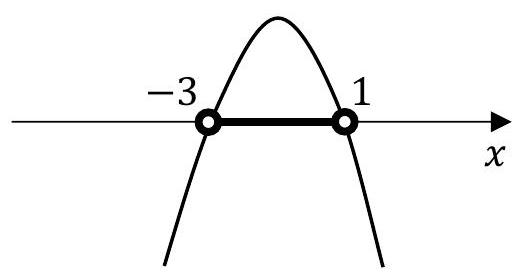
\includegraphics[max width=\textwidth, center]{2025_02_07_83b95a6405af75d2626bg-17}
\end{itemize}

1 pkt - obliczenie lub podanie pierwiastków trójmianu kwadratowego $-x^{2}-2 x+3$ :

$$
\begin{aligned}
& x_{1}=1 \text { oraz } x_{2}=-3 \\
& A L B O
\end{aligned}
$$

\begin{itemize}
  \item odczytanie z wykresu funkcji $f(x)=-x^{2}-2 x+3$ i zapisanie miejsc zerowych $x_{1}=1$ oraz $x_{2}=-3$.\\
0 pkt - rozwiązanie, w którym zastosowano niepoprawną metodę, albo brak rozwiązania.
\end{itemize}

\section*{Uwagi:}
\begin{enumerate}
  \item Jeżeli zdający, realizując pierwszy etap rozwiązania zadania, popełni błędy (ale otrzyma dwa różne pierwiastki) i konsekwentnie do popełnionych błędów zapisze zbiór rozwiązań nierówności, to otrzymuje 1 punkt za całe rozwiązanie.
  \item Jeżeli zdający wyznacza pierwiastki trójmianu kwadratowego w przypadku, gdy błędnie obliczony przez zdającego wyróżnik $\Delta$ jest ujemny, to otrzymuje $\mathbf{0}$ punktów za całe rozwiązanie.
  \item Jeżeli zdający, rozpoczynając realizację pierwszego etapu rozwiązania, rozpatruje inny niż podany w zadaniu trójmian kwadratowy, który nie wynika z błędu przekształcenia (np. $x^{2}-2 x$ ), i w konsekwencji rozpatruje inną nierówność (np. $x^{2}-2 x>0$ ), to oznacza, że nie podjął realizacji 1. etapu rozwiązania i otrzymuje 0 punktów za całe rozwiązanie.
  \item Akceptowane jest zapisanie pierwiastków trójmianu w postaci $a+b \sqrt{c}$, gdzie $a, b, c$ są liczbami wymiernymi.
  \item Jeżeli zdający poda zbiór rozwiązań w postaci graficznej z poprawnie zaznaczonymi końcami przedziałów oraz zapisze: $x \in\langle-3,1\rangle$, to otrzymuje 1 punkt za całe rozwiązanie.
\end{enumerate}

\section*{Kryteria uwzględniające specyficzne trudności w uczeniu się matematyki}
Jeśli zdający pomyli porządek liczb na osi liczbowej, np. zapisze zbiór rozwiązań nierówności w postaci $(1,-3)$, to otrzymuje 2 punkty.

\section*{Przykładowe pełne rozwiązanie}
Zapisujemy nierówność w postaci $-x^{2}-2 x+3>0$ i obliczamy pierwiastki trójmianu $-x^{2}-2 x+3$.\\
Obliczamy wyróżnik trójmianu: $\Delta=16$\\
i obliczamy jego pierwiastki: $x_{1}=-3$ oraz $x_{2}=1$\\
ALBO\\
podajemy pierwiastki trójmianu bezpośrednio, zapisując je lub zaznaczając je na wykresie:\\
$x_{1}=-3$ oraz $x_{2}=1$.\\
Podajemy zbiór rozwiązań nierówności: $(-3,1)$ lub $x \in(-3,1)$, lub zaznaczamy zbiór rozwiązań na osi liczbowej:\\
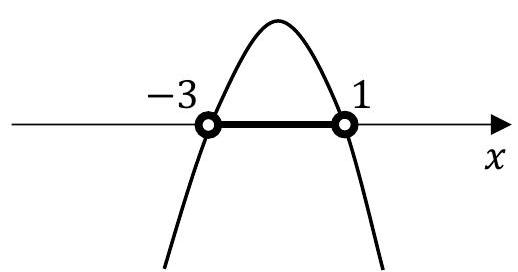
\includegraphics[max width=\textwidth, center]{2025_02_07_83b95a6405af75d2626bg-18}

Zadanie 31. (0-2)

\begin{center}
\begin{tabular}{|l|l|}
\hline
\multicolumn{2}{|c|}{Wymagania egzaminacyjne 2023 i 2024} \\
\hline
\multicolumn{1}{|c|}{Wymaganie ogólne} & \multicolumn{1}{|c|}{Wymaganie szczegółowe} \\
\hline
III. Modelowanie matematyczne. & \begin{tabular}{l}
Zdający: \\
5.3) stosuje wzór na $n$-ty wyraz i na sumę \\
$n$ początkowych wyrazów ciągu \\
arytmetycznego. \\
\end{tabular} \\
\hline
\end{tabular}
\end{center}

\section*{Zasady oceniania}
2 pkt - zastosowanie poprawnej metody i obliczenie pierwszej raty: 750 zł.\\
1 pkt - zastosowanie wzoru na sumę $n$ początkowych wyrazów ciągu arytmetycznego\\
i zapisanie równania z niewiadomą $a_{1}$ (pierwszą ratą):\\
$\frac{2 a_{1}+17 \cdot(-30)}{2} \cdot 18=8910$\\
ALBO

\begin{itemize}
  \item zastosowanie wzoru na sumę $n$ początkowych wyrazów ciągu arytmetycznego oraz zapisanie równania $z$ niewiadomą $a_{1}$ :\\
$\frac{2 a_{1}+17 \cdot 30}{2} \cdot 18=8910$ i zapisanie, że $a_{1}$ jest ostannią ratą,\\
ALBO
  \item zapisanie równania\\
$a_{1}+\left(a_{1}-30\right)+\left(a_{1}-2 \cdot 30\right)+\left(a_{1}-3 \cdot 30\right)+\cdots+\left(a_{1}-17 \cdot 30\right)=8910$, gdzie $a_{1}$ jest pierwszą ratą, lub równania\\
$a_{1}+\left(a_{1}+30\right)+\left(a_{1}+2 \cdot 30\right)+\left(a_{1}+3 \cdot 30\right)+\cdots+\left(a_{1}+17 \cdot 30\right)=8910$\\
(łącznie z zapisem, że $a_{1}$ jest ostatnią ratą),\\
ALBO
  \item zapisanie zależności między pierwszą $\left(a_{1}\right)$ i ostatnią ratą ( $a_{18}$ ), np.\\
$a_{1}+a_{18}=8910: 9$ albo $a_{18}=a_{1}-17 \cdot 30$ itp.,\\
ALBO
  \item rozpatrzenie osiemnastowyrazowego ciągu arytmetycznego o różnicy (-30) lub 30 i zapisanie co najmniej pierwszego oraz ostatniego wyrazu tego ciągu, np .\\
( $x, x-30, x-60, \ldots, x-510$ ) dla dowolnego $x$ (np. jak w sposobie V ), ALBO
  \item zapisanie układu równań, z którego można obliczyć jedną z rat, np.\\
$\frac{a_{9}+a_{10}}{2}=495$ i $a_{10}=a_{9}-30$.\\
0 pkt - rozwiązanie, w którym zastosowano niepoprawną metodę, albo brak rozwiązania.
\end{itemize}

\section*{Uwagi:}
\begin{enumerate}
  \item Jeżeli zdający myli ciąg arytmetyczny z geometrycznym, to otrzymuje $\mathbf{0}$ punktów za całe rozwiązanie, o ile nie nabył prawa do innej liczby punktów.
  \item Jeżeli zdający zapisze tylko 750 zł, to otrzymuje 1 punkt za całe rozwiązanie.
  \item Jeżeli zdający rozważa ciąg arytmetyczny o różnicy $r=30$, obliczy $a_{1}=240$ i nie interpretuje $a_{1}$ jako ostatniej raty, to może otrzymać co najwyżej 1 punkt za całe rozwiązanie.
  \item Jeżeli zdający błędnie interpretuje liczbę 8910 jako wyraz ciągu rat, to otrzymuje 0 punktów za całe rozwiązanie.
\end{enumerate}

\section*{Przykładowe pełne rozwiązania}
Sposób I\\
Kolejne raty tworzą ciąg arytmetyczny, w którym $S_{18}=8910$ i $r=-30$. Korzystamy ze wzoru na sumę $n$ początkowych wyrazów ciągu arytmetycznego i otrzymujemy równanie

$$
\frac{2 a_{1}+17 \cdot(-30)}{2} \cdot 18=8910
$$

Przekształcając to równanie równoważnie, otrzymujemy

$$
\begin{gathered}
9\left(2 a_{1}-510\right)=8910 \\
2 a_{1}-510=990 \\
a_{1}=750
\end{gathered}
$$

Pierwsza rata była równa 750 zł.

Sposób II\\
Przyjmujemy, że kolejne (licząc od końca) raty tworzą ciąg arytmetyczny, w którym $S_{18}=8910$ i $r=30$. Korzystamy ze wzoru na sumę $n$ początkowych wyrazów ciągu arytmetycznego i otrzymujemy równanie

$$
\frac{2 a_{1}+17 \cdot 30}{2} \cdot 18=8910
$$

Przekształcając to równanie równoważnie, otrzymujemy

$$
\begin{gathered}
9\left(2 a_{1}+510\right)=8910 \\
2 a_{1}+510=990 \\
a_{1}=240
\end{gathered}
$$

Ostatnia rata była równa 240 zł.\\
Obliczamy wysokość pierwszej raty

$$
a_{18}=240+17 \cdot 30=750
$$

Pierwsza rata była równa 750 zł.

\section*{Sposób III}
Kolejne kwoty, o które pomniejszana jest pierwsza rata, tworzą ciąg arytmetyczny, w którym różnica jest równa 30 . Wtedy osiemnasta rata jest mniejsza od pierwszej raty o kwotę $(18-1) \cdot 30=510$ zł.

Stąd

$$
\begin{gathered}
a_{1}+\left(a_{1}-30\right)+\left(a_{1}-60\right)+\left(a_{1}-90\right)+\ldots+\left(a_{1}-510\right)=8910 \\
18 a_{1}-(30+60+90+\ldots+510)=8910
\end{gathered}
$$

gdzie suma siedemnastu liczb $30+60+90+\ldots+510$ jest równa

$$
\frac{30+510}{2} \cdot 17=4590
$$

Zatem

$$
\begin{gathered}
18 a_{1}-4590=8910 \\
18 a_{1}=13500 \\
a_{1}=750
\end{gathered}
$$

Pierwsza rata była równa 750 zł.

\section*{Sposób IV}
Kolejne raty tworzą ciąg arytmetyczny, zatem

$$
a_{1}+a_{18}=a_{2}+a_{17}=a_{3}+a_{16}=\ldots=a_{9}+a_{10}
$$

Obliczamy wartość pojedynczej sumy

$$
a_{1}+a_{18}=8910: 9=990
$$

Korzystając ze wzoru na $n$-ty wyraz ciągu arytmetycznego, mamy

$$
\begin{gathered}
a_{1}+a_{1}-17 \cdot 30=990 \\
2 a_{1}=990+510 \\
a_{1}=750
\end{gathered}
$$

Pierwsza rata była równa 750 zł.

\section*{Sposób V}
Przyjmujemy, że pierwsza rata była równa 1000 zł. Wtedy kolejne raty są równe:

$$
970 \mathrm{zł}, 940 \mathrm{zł}, \ldots, 490 \mathrm{zł} .
$$

Suma wszystkich rat jest równa 13410 zł i przewyższa kwotę z warunków zadania o 4500 zł.

Obliczamy, o ile należy zmniejszyć każdą ratę:

$$
\begin{gathered}
4500: 18=250 \\
1000-250=750
\end{gathered}
$$

Pierwsza rata była równa 750 zł.

\section*{Sposób VI}
Kolejne raty są wyrazami osiemnastowyrazowego ciągu arytmetycznego ( $a_{n}$ ) o różnicy $r=-30$. Obliczymy dowolną ratę (np. dziewiątą), korzystając z własności tego ciągu:

$$
\begin{aligned}
\left\{\begin{array}{c}
\left(a_{9}+a_{10}\right) \cdot 9=8910 \\
a_{10}=a_{9}-30
\end{array}\right. & \left\{\begin{array}{l}
a_{9}+a_{10}=990 \\
a_{9}-a_{10}=30
\end{array}\right. \\
2 a_{9}=1020 & a_{9}=510
\end{aligned}
$$

Zatem

$$
a_{1}=a_{9}-8 \cdot(-30)=510+240=750
$$

Zadanie 32. (0-2)

\begin{center}
\begin{tabular}{|l|l|}
\hline
\multicolumn{2}{|c|}{Wymagania egzaminacyjne 2023 i 2024} \\
\hline
\multicolumn{1}{|c|}{Wymaganie ogólne} & \multicolumn{1}{|c|}{Wymaganie szczegółowe} \\
\hline
V. Rozumowanie i argumentacja. & \begin{tabular}{l}
Zdający: \\
2. užywa wzorów skróconego mnożenia na \\
$(a \pm b)^{2}$ oraz $a^{2}-b^{2}$. \\
\end{tabular} \\
\hline
\end{tabular}
\end{center}

\section*{Zasady oceniania}
2 pkt - przekształcenie nierówności $x^{2}+y^{2}+5>2 x+4 y$ do postaci $(x-1)^{2}+(y-2)^{2}>0$ oraz powołanie się na założenie i stwierdzenie, że $(x-1)^{2}$ jest liczbą dodatnią i suma $(x-1)^{2}+(y-2)^{2}$ jest liczbą dodatnią ALBO

\begin{itemize}
  \item obliczenie wyróżnika trójmianu kwadratowego $x^{2}-2 x+\left(y^{2}-4 y+5\right)$ zmiennej $x$ oraz uzasadnienie, że jest on niedodatni, oraz uzasadnienie prawdziwości nierówności $x^{2}+y^{2}+5>2 x+4 y$ dla $y=2$, ALBO
  \item obliczenie wyróżnika trójmianu kwadratowego $y^{2}-4 y+\left(x^{2}-2 x+5\right)$ zmiennej $y$ oraz uzasadnienie, że ten wyróżnik jest ujemny dla każdego $x \neq 1$, ALBO
  \item przekształcenie nierówności do postaci $f(x)>g(y)$ oraz poprawne uzasadnienie prawdziwości nierówności $f(x)>g(y)$ dla każdego $x \neq 1$ i $y \in \mathbb{R}$ na podstawie analizy zbiorów wartości obu funkcji.
\end{itemize}

1 pkt - przekształcenie nierówności $x^{2}+y^{2}+5>2 x+4 y$ do postaci\\
$(x-1)^{2}+(y-2)^{2}>0$\\
ALBO

\begin{itemize}
  \item obliczenie wyróżnika $\Delta$ trójmianu kwadratowego $x^{2}-2 x+\left(y^{2}-4 y+5\right)$\\
zmiennej $x$ oraz przekształcenie tego wyróżnika do postaci $\Delta=-(2 y-4)^{2}$ bądź $\Delta=-4(y-2)^{2}$ lub (zamiast przekształcenia wyróżnika) zbadanie znaku tego wyróżnika (np. obliczenie wyróżnika trójmianu $-4 y^{2}+16 y-16$ ), ALBO
  \item obliczenie wyróżnika $\Delta$ trójmianu kwadratowego $y^{2}-4 y+\left(x^{2}-2 x+5\right)$ zmiennej $y$ oraz przekształcenie tego wyróżnika do postaci $\Delta=-(2 x-2)^{2}$ bądź $\Delta=-4(x-1)^{2}$ lub (zamiast przekształcenia wyróżnika) zbadanie znaku tego wyróżnika ( np . obliczenie wyróżnika trójmianu $-4 x^{2}+8 x-4$ ),\\
ALBO
  \item przekształcenie nierówności do postaci $f(x)>g(y)$ oraz zbadanie zbioru wartości jednej z funkcji: $f$ albo $g$.\\
0 pkt - rozwiązanie, w którym zastosowano niepoprawną metodę, albo brak rozwiązania.
\end{itemize}

\section*{Uwaga:}
Jeśli zdający sprawdza prawdziwość nierówności tylko dla wybranych wartości $x$ i $y$, to otrzymuje $\mathbf{0}$ punktów za całe rozwiązanie.

\section*{Przykładowe pełne rozwiązania}
\section*{Sposób I}
Przekształcamy nierówność $x^{2}+y^{2}+5>2 x+4 y$ w sposób równoważny:

$$
x^{2}-2 x+1+y^{2}-4 y+4>0
$$

Zauważamy, że lewą stronę nierówności można zapisać w postaci sumy dwóch kwadratów

$$
(x-1)^{2}+(y-2)^{2}>0
$$

Z założenia wiadomo, że $x \neq 1$, więc $(x-1)^{2}$ jest liczbą dodatnią. Liczba $(y-2)^{2}$ jest liczbą nieujemną, zatem suma $(x-1)^{2}+(y-2)^{2}$ jest liczbą dodatnią.\\
To należało wykazać.\\
Sposób II (trójmian kwadratowy zmiennej $x$ z parametrem y) Przekształcamy równoważnie nierówność $x^{2}+y^{2}+5>2 x+4 y$ i otrzymujemy $x^{2}-2 x+y^{2}-4 y+5>0$.\\
Wyrażenie $x^{2}-2 x+\left(y^{2}-4 y+5\right)$ traktujemy jako trójmian kwadratowy zmiennej $x$.\\
Obliczamy wyróżnik $\Delta$ trójmianu:

$$
\begin{gathered}
\Delta=(-2)^{2}-4 \cdot\left(y^{2}-4 y+5\right) \\
\Delta=4-4 y^{2}+16 y-20 \\
\Delta=-4\left(y^{2}-4 y+4\right) \\
\Delta=-4(y-2)^{2}
\end{gathered}
$$

Gdy $y \neq 2$, to $\Delta<0$ i funkcja kwadratowa $f(x)=x^{2}-2 x+\left(y^{2}-4 y+5\right)$ zmiennej $x$ nie ma miejsc zerowych, a ponieważ współczynnik przy drugiej potędze zmiennej jest dodatni, więc żaden fragment wykresu funkcji $f$ nie leży poniżej osi odciętych. Zatem funkcja przyjmuje tylko wartości dodatnie.

Gdy $y=2$, to $\Delta=0$ i funkcja $f$ ma dokładnie jedno miejsce zerowe: $x=1$. Ponieważ współczynnik przy drugiej potędze zmiennej jest dodatni, więc żaden fragment wykresu\\
funkcji $f$ nie leży poniżej osi odciętych. Zatem funkcja $f$ przyjmuje wartości dodatnie dla każdego $x \neq 1$.

Oznacza to, że dla każdej liczby rzeczywistej $x \neq 1$ i dla każdej liczby rzeczywistej $y$ nierówność $x^{2}-2 x+\left(y^{2}-4 y+5\right)>0$ jest prawdziwa.\\
Zatem nierówność $x^{2}+y^{2}+5>2 x+4 y$ również jest prawdziwa dla każdej liczby rzeczywistej $x \neq 1$ i dla każdej liczby rzeczywistej $y$. To należało wykazać.

\section*{Sposób III (poprzez analize zbioru wartości dwóch funkcii)}
Przekształcamy równoważnie nierówność $x^{2}+y^{2}+5>2 x+4 y$ do postaci\\
$f(x)>g(y)$, następnie analizujemy zbiory wartości funkcji $f$ (określonej dla każdej liczby rzeczywistej $x \neq 1$ ) oraz funkcji $g$ (określonej dla każdej liczby rzeczywistej $y$ ). Takie przekształcenie równoważne nierówności można wykonać na różne sposoby, np. tak:

$$
x^{2}-2 x+1>-y^{2}+4 y-4 \quad \text { oraz } \quad x \neq 1 \text { i } y \in \mathbb{R}
$$

Otrzymaną postać nierówności przekształcamy do postaci

$$
(x-1)^{2}>-(y-2)^{2} \quad \text { oraz } \quad x \neq 1 \text { i } y \in \mathbb{R}
$$

Rozważamy funkcje $f$ i $g$ takie, że

$$
f(x)=(x-1)^{2} \quad \text { dla } \quad x \neq 1 \quad \text { oraz } \quad g(y)=-(y-2)^{2} \quad \text { dla } \quad y \in \mathbb{R}
$$

Zbiorami wartości tych funkcji są przedziały: $Z W_{f}=(0,+\infty)$ oraz $Z W_{g}=(-\infty, 0]$. Zauważmy, że każda wartość funkcji $f$ jest większa od każdej wartości funkcji $g$. To oznacza, że dla każdej liczby rzeczywistej $x \neq 1$ oraz dla każdej liczby rzeczywistej $y$ zachodzi nierówność $f(x)>g(y)$.\\
Zatem nierówność $x^{2}+y^{2}+5>2 x+4 y$ jest prawdziwa dla każdej liczby rzeczywistej $x \neq 1$ i dla każdej liczby rzeczywistej $y$. To należało wykazać.

\section*{Zadanie 33. (0-2)}
\begin{center}
\begin{tabular}{|l|l|}
\hline
\multicolumn{2}{|c|}{Wymagania egzaminacyjne 2023 i 2024} \\
\hline
\multicolumn{1}{|c|}{Wymaganie ogólne} & \multicolumn{1}{c|}{Wymagania szczegółowe} \\
\hline
IV. Użycie i tworzenie strategii. & Zdający: \\
 & G10.7) stosuje twierdzenie Pitagorasa. \\
 & 7.3) rozpoznaje trójkąty podobne \\
 & i wykorzystuje cechy podobieństwa \\
 & trójkątów. \\
\hline
\end{tabular}
\end{center}

\section*{Zasady oceniania}
2 pkt - poprawna metoda i obliczenie pola trójkąta $T_{2}: P_{2}=120$.\\
1 pkt - wykorzystanie podobieństwa trójkątów i zapisanie układu równań/równania pozwalającego obliczyć długości przyprostokątnych trójkąta $T_{2}$, np.\\
$\frac{a_{2}}{b_{2}}=\frac{12}{5}$ i $a_{2}^{2}+b_{2}^{2}=26^{2},(12 x)^{2}+(5 x)^{2}=26^{2}$\\
ALBO

\begin{itemize}
  \item zapisanie stosunku pól trójkątów $T_{1}$ i $T_{2}: \frac{P_{1}}{P_{2}}=\left(\frac{|B C|}{26}\right)^{2}$ (lub $\frac{P_{2}}{P_{1}}=\left(\frac{26}{|B C|}\right)^{2}$ ) oraz obliczenie długości odcinka $B C$ : $|B C|=13$, ALBO
  \item obliczenie/zapisanie skali podobieństwa trójkątów, np. $k=\frac{|E F|}{|B C|}=2$\\
(lub $k=\frac{|B C|}{|E F|}=\frac{1}{2}$ ),\\
ALBO
  \item obliczenie/zapisanie długości przyprostokątnych trójkąta $T_{2}: 10,24$, ALBO
  \item obliczenie długości $c_{1}$ przeciwprostokątnej trójkąta $T_{1}$ oraz zapisanie układu równań pozwalającego obliczyć długości $a_{2}, b_{2}$ przyprostokątnych trójkąta $T_{2}$, np.
\end{itemize}

$$
c_{1}=13 ; \frac{13}{12}=\frac{26}{a_{2}} ; \frac{13}{5}=\frac{26}{b_{2}} .
$$

0 pkt - rozwiązanie, w którym zastosowano niepoprawną metodę, albo brak rozwiązania.

\section*{Przykładowe pełne rozwiązania}
\section*{Sposób l}
Długości przyprostokątnych trójkątów $T_{1}$ i $T_{2}$ oznaczymy odpowiednio jako: $a_{1}, b_{1}$ oraz $a_{2}, b_{2}$. Z podobieństwa trójkątów $T_{1}$ i $T_{2}$ wynika, że stosunki odpowiednich boków są równe:

$$
\frac{a_{2}}{b_{2}}=\frac{a_{1}}{b_{1}} \text { gdzie } a_{1}=12, \quad b_{1}=5
$$

Zatem

$$
\frac{a_{2}}{b_{2}}=\frac{12}{5} \text { więc } \quad b_{2}=\frac{5}{12} a_{2}
$$

Z twierdzenia Pitagorasa dla trójkąta $T_{2}$ mamy:

$$
\begin{gathered}
a_{2}^{2}+b_{2}^{2}=26^{2} \\
a_{2}^{2}+\left(\frac{5}{12}\right)^{2} a_{2}^{2}=26^{2} \\
\frac{169}{144} a_{2}^{2}=26^{2} \\
a_{2}=\sqrt{\frac{144}{169}} \cdot 26=24
\end{gathered}
$$

Zatem $b_{2}=\frac{5}{12} \cdot 24=10$.\\
Obliczamy pole trójkąta $T_{2}$ :

$$
P_{2}=\frac{1}{2} \cdot a_{2} \cdot b_{2}=\frac{1}{2} \cdot 24 \cdot 10=120
$$

\section*{Sposób II}
Oznaczamy wierzchołki trójkąta $T_{1}$ przez $A, B, C$, gdzie $B C$ jest przeciwprostokątną tego trójkąta, $|A B|=12$ i $|A C|=5$. Oznaczamy wierzchołki trójkąta $T_{2}$ przez $D, E, F$, gdzie $E F$ jest przeciwprostokątną tego trójkąta.\\
$Z$ twierdzenia Pitagorasa dla trójkąta $T_{1}$ mamy

$$
\begin{gathered}
|A B|^{2}+|A C|^{2}=|B C|^{2} \\
12^{2}+5^{2}=|B C|^{2} \\
|B C|^{2}=169 \\
|B C|=13
\end{gathered}
$$

\begin{center}
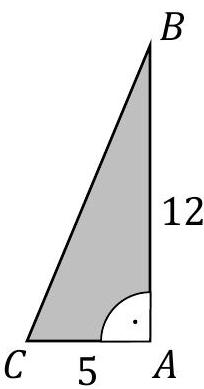
\includegraphics[max width=\textwidth]{2025_02_07_83b95a6405af75d2626bg-26}
\end{center}

Obliczamy skalę podobieństwa trójkąta $T_{2}$ do trójkąta $T_{1}$ :

$$
k=\frac{|E F|}{|B C|}=\frac{26}{13}=2
$$

Obliczamy długości przyprostokątnych trójkąta $T_{2}$ :

$$
\begin{gathered}
|D E|=2 \cdot|A B|=2 \cdot 12=24 \\
|D F|=2 \cdot|A C|=2 \cdot 5=10
\end{gathered}
$$

Obliczamy pole trójkąta $T_{2}$ :

$$
P_{2}=\frac{1}{2} \cdot|D E| \cdot|D F|=\frac{1}{2} \cdot 24 \cdot 10=120
$$

\section*{Sposób III}
Oznaczamy wierzchołki trójkąta $T_{1}$ przez $A, B, C$, gdzie $B C$ jest przeciwprostokątną tego trójkąta, $|A B|=12$ i $|A C|=5$. Oznaczamy wierzchołki trójkąta $T_{2}$ przez $D, E, F$, gdzie $E F$ jest przeciwprostokątną tego trójkąta.

Z twierdzenia Pitagorasa dla trójkąta $T_{1}$ mamy

$$
\begin{gathered}
|A B|^{2}+|A C|^{2}=|B C|^{2} \\
12^{2}+5^{2}=|B C|^{2} \\
|B C|^{2}=169 \\
|B C|=13
\end{gathered}
$$

Obliczamy skalę podobieństwa trójkąta $T_{2}$ do trójkąta $T_{1}$ :

$$
k=\frac{|E F|}{|B C|}=\frac{26}{13}=2
$$

\begin{center}
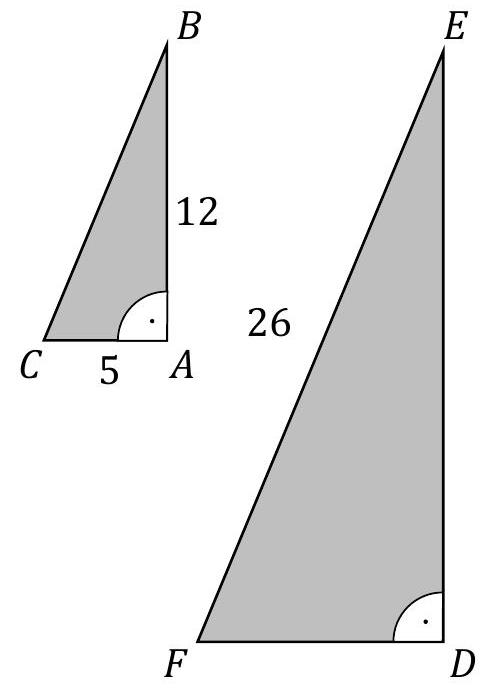
\includegraphics[max width=\textwidth]{2025_02_07_83b95a6405af75d2626bg-26(1)}
\end{center}

Obliczamy pole $P_{1}$ trójkąta $T_{1}$ :

$$
P_{1}=\frac{1}{2} \cdot|A B| \cdot|A C|=\frac{1}{2} \cdot 12 \cdot 5=30
$$

Korzystając z tego, że stosunek pól figur podobnych jest równy kwadratowi skali podobieństwa, obliczamy pole $P_{2}$ trójkąta $T_{2}$ :

$$
\frac{P_{2}}{P_{1}}=k^{2}
$$

Zatem

$$
P_{2}=k^{2} \cdot P_{1}=2^{2} \cdot 30=120
$$

Zadanie 34. (0-2)

\begin{center}
\begin{tabular}{|l|l|}
\hline
\multicolumn{2}{|c|}{Wymagania egzaminacyjne 2023 i 2024} \\
\hline
\multicolumn{1}{|c|}{Wymaganie ogólne} & \multicolumn{1}{c|}{Wymagania szczegółowe} \\
\hline
II. Wykorzystanie i interpretowanie & Zdający: \\
reprezentacji. & 8.1) wyznacza równanie prostej \\
 & przechodzacej przez dwa dane punkty \\
 & (w postaci kierunkowej lub ogólnej); \\
 & 8.5) wyznacza współrzędne środka odcinka; \\
 & 8.3) wyznacza równanie prostej, która jest \\
 & [...] prostopadła do prostej danej w postaci \\
 & kierunkowej i przechodzi przez dany punkt. \\
\hline
\end{tabular}
\end{center}

\section*{Zasady oceniania}
2 pkt - wyznaczenie i zapisanie równania prostej zawierającej przekątną $B D$ (w postaci równania stopnia pierwszego $z$ dwiema niewiadomymi) np. $y=-\frac{4}{3} x-\frac{13}{3}$.\\
1 pkt - obliczenie współrzędnej punktu $S$ oraz obliczenie współczynnika kierunkowego prostej $A C$ (lub zapisanie równania prostej $A C$ ): $S=(-4,1)$ oraz $\frac{3}{4}$ ALBO

\begin{itemize}
  \item wyznaczenie współczynnika kierunkowego prostej $B D:\left(-\frac{4}{3}\right)$,
\end{itemize}

\section*{ALBO}
\begin{itemize}
  \item zapisanie równości $|P A|=|P C|$ wynikającej z własności symetralnej (gdzie $P$ jest punktem leżącym na symetralnej odcinka $A C$ ) lub zapisanie równania postaci $\sqrt{(x+8)^{2}+(y+2)^{2}}=\sqrt{(x-0)^{2}+(y-4)^{2}}$\\
ALBO
  \item wyznaczenie współrzędnych punktów $B$ i $D$ (lub jednego z nich i punktu $S$ ), z wykorzystaniem punktów kratowych.\\
0 pkt - rozwiązanie, w którym zastosowano niepoprawną metodę, albo brak rozwiązania.
\end{itemize}

\section*{Przykładowe pełne rozwiązanie}
Ponieważ przekątne w kwadracie dzielą się na połowy, szukamy środka odcinka $A C$ :

$$
S=\left(\frac{x_{A}+x_{C}}{2}, \frac{y_{A}+y_{C}}{2}\right)=\left(\frac{-8+0}{2}, \frac{-2+4}{2}\right)=(-4,1)
$$

Korzystając ze wzoru $\left(y-y_{A}\right)\left(x_{C}-x_{A}\right)-\left(y_{C}-y_{A}\right)\left(x-x_{A}\right)=0$, wyznaczamy równanie prostej $A C$ :

$$
\begin{gathered}
(y-(-2))(0-(-8))-(4-(-2))(x-(-8))=0 \\
(y+2) \cdot 8-6 \cdot(x+8)=0 \\
8 y=6 x+32 \\
y=\frac{3}{4} x+4
\end{gathered}
$$

Prosta zawierająca przekątną $B D$ jest prostopadła do prostej $A C$, zatem jej współczynnik kierunkowy jest równy $\left(-\frac{4}{3}\right)$.

Obliczamy współczynnik $b$ równania kierunkowego prostej $B D$, podstawiając do wzoru $y=-\frac{4}{3} x+b$ współrzędne punktu $S=(-4,1)$ :

$$
\begin{gathered}
1=-\frac{4}{3} \cdot(-4)+b \\
b=-\frac{13}{3}
\end{gathered}
$$

Prosta zawierająca przekątną $B D$ kwadratu $A B C D$ ma postać $y=-\frac{4}{3} x-\frac{13}{3}$.

\section*{Uwaga:}
Równanie prostej, która zawiera przekątną $B D$ kwadratu $A B C D$, można wyznaczyć z równości wynikającej z własności symetralnej odcinka $A C$.\\
Niech $P=(x, y)$ będzie punktem leżącym na symetralnej odcinka $A C$.\\
Wtedy:

$$
\begin{gathered}
|P A|=|P C| \\
\sqrt{(x+8)^{2}+(y+2)^{2}}=\sqrt{(x-0)^{2}+(y-4)^{2}} \\
(x+8)^{2}+(y+2)^{2}=(x-0)^{2}+(y-4)^{2} \\
x^{2}+16 x+64+y^{2}+4 y+4=x^{2}+y^{2}-8 y+16 \\
12 y=-16 x-68+16 \\
y=-\frac{4}{3} x-\frac{13}{3}
\end{gathered}
$$

Zadanie 35. (0-2)

\begin{center}
\begin{tabular}{|l|l|}
\hline
\multicolumn{2}{|c|}{Wymagania egzaminacyjne 2023 i 2024} \\
\hline
\multicolumn{1}{|c|}{Wymaganie ogólne} & \multicolumn{1}{c|}{Wymaganie szczegółowe} \\
\hline
III. Modelowanie matematyczne. & Zdający: \\
 & 10.2) oblicza prawdopodobieństwa \\
 & w prostych sytuacjach, stosując klasyczną \\
 & definicję prawdopodobieństwa. \\
\hline
\end{tabular}
\end{center}

\section*{Zasady oceniania}
2 pkt - zastosowanie poprawnej metody obliczenia prawdopodobieństwa zdarzenia $A$ i uzyskanie poprawnego wyniku: $P(A)=\frac{6}{64}$.\\
1 pkt - wypisanie wszystkich zdarzeń elementarnych lub obliczenie/podanie liczby tych zdarzeń: $|\Omega|=8 \cdot 8$ lub sporządzenie tabeli o 64 polach odpowiadających zdarzeniom elementarnym, z których co najmniej jedno pole jest wypełnione, lub sporządzenie pełnego drzewa stochastycznego ALBO

\begin{itemize}
  \item wypisanie (zaznaczenie w tabeli) wszystkich zdarzeń elementarnych sprzyjających zdarzeniu $A$ i niewypisanie żadnego niewłaściwego:\\
$(3,5),(5,3),(6,5),(5,6),(5,9),(9,5)$, ALBO
  \item podanie liczby wszystkich zdarzeń elementarnych sprzyjających zdarzeniu $A$ : $|A|=6$, jeśli nie została otrzymana w wyniku zastosowania błędnej metody, ALBO
  \item sporządzenie fragmentu drzewa stochastycznego, które zawiera wszystkie gałęzie sprzyjające zdarzeniu $A$ oraz zapisanie prawdopodobieństwa $\frac{1}{8}$ na co najmniej jednym odcinku każdego z etapów doświadczenia, ALBO
  \item podanie prawdopodobieństwa jednoelementowego zdarzenia (elementarnego): $\frac{1}{64}$, ALBO
  \item zapisanie tylko $P(A)=\frac{6}{64}$.
\end{itemize}

0 pkt - rozwiązanie, w którym zastosowano niepoprawną metodę, albo brak rozwiązania.

\section*{Uwaga:}
Jeżeli zdający zapisuje tylko liczby 6 lub 64 i z rozwiązania nie wynika znaczenie tych liczb, to otrzymuje $\mathbf{0}$ punktów za całe rozwiązanie.

\section*{Przykładowe pełne rozwiązania}
Sposób 1\\
Zbiór wszystkich zdarzeń elementarnych obrazuje tabela $8 \times 8$, co oznacza, że moc zbioru $\Omega$ jest równa 64.

W tabeli zaznaczamy iloczyny podzielne przez 15 .

\begin{center}
\begin{tabular}{|l|l|l|l|l|l|l|l|l|}
\hline
 & 2 & 3 & 4 & 5 & 6 & 7 & 8 & 9 \\
\hline
2 &  &  &  &  &  &  &  &  \\
\hline
3 &  &  &  & $\times$ &  &  &  &  \\
\hline
4 &  &  &  &  &  &  &  &  \\
\hline
5 &  & $\times$ &  &  & $\times$ &  &  & $\times$ \\
\hline
6 &  &  &  & $\times$ &  &  &  &  \\
\hline
7 &  &  &  &  &  &  &  &  \\
\hline
8 &  &  &  &  &  &  &  &  \\
\hline
9 &  &  &  & $\times$ &  &  &  &  \\
\hline
\end{tabular}
\end{center}

Zdarzeń sprzyjających wylosowaniu liczb, których iloczyn jest podzielny przez 15, jest 6. Zatem prawdopodobieństwo zdarzenia polegającego na wylosowaniu liczb, których iloczyn jest podzielny przez 15 , jest równe $\frac{6}{64}$.

\section*{Sposób II (drzewo stochastyczne)}
Rysujemy fragment drzewa stochastycznego rozważanego doświadczenia z uwzględnieniem wszystkich istotnych gałęzi.\\
Oznaczamy przez $A$ zdarzenie polegające na tym, że iloczyn wylosowanych liczb jest podzielny przez 15.\\
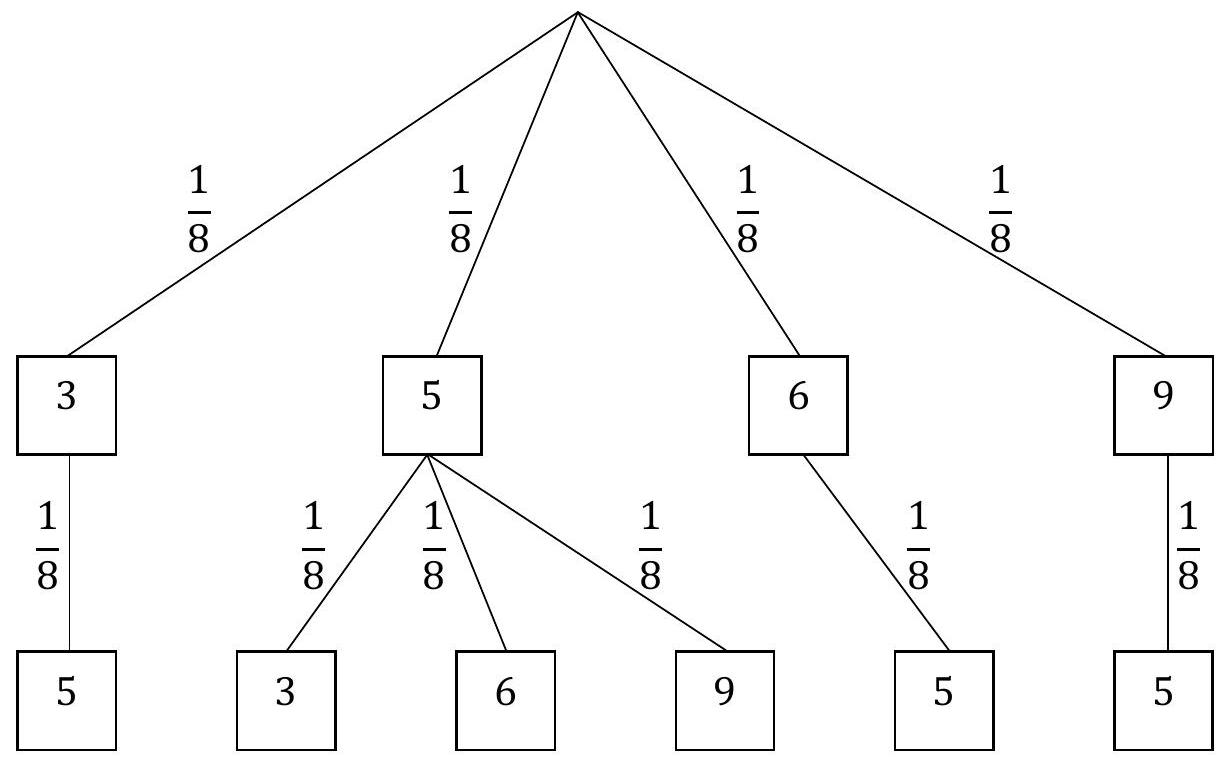
\includegraphics[max width=\textwidth, center]{2025_02_07_83b95a6405af75d2626bg-30}

Prawdopodobieństwo zdarzenia $A$ jest równe

$$
P(A)=\frac{1}{8} \cdot \frac{1}{8}+\frac{1}{8} \cdot \frac{1}{8}+\frac{1}{8} \cdot \frac{1}{8}+\frac{1}{8} \cdot \frac{1}{8}+\frac{1}{8} \cdot \frac{1}{8}+\frac{1}{8} \cdot \frac{1}{8}=\frac{6}{64}
$$

\section*{Sposób III}
Zbiór wszystkich zdarzeń elementarnych $\Omega$ to zbiór par uporządkowanych elementów ze zbioru 8-elementowego, zatem moc zbioru $\Omega$ jest równa $|\Omega|=8 \cdot 8=64$.\\
Oznaczamy przez $A$ zdarzenie polegające na tym, że iloczyn wylosowanych liczb jest podzielny przez 15.\\
Wielokrotności liczby 15 , które mogą być iloczynami elementów ze zbioru $\Omega$, to $15,30,45$. Wyznaczamy iloczyny, które spełniają powyższy warunek:\\
$15=3 \cdot 5=5 \cdot 3$ - dwa iloczyny - dwa zdarzenia elementarne: $(3,5)$ oraz $(5,3)$,\\
$30=6 \cdot 5=5 \cdot 6-$ dwa iloczyny - dwa zdarzenia elementarne: $(6,5)$ oraz $(5,6)$,\\
$45=9 \cdot 5=5 \cdot 9-$ dwa iloczyny - dwa zdarzenia elementarne: $(9,5)$ oraz $(5,9)$.\\
Sprzyjających zdarzeń elementarnych jest 6 , więc $P(A)=\frac{6}{64}$.

Zadanie 36. (0-5)

\begin{center}
\begin{tabular}{|l|l|}
\hline
\multicolumn{2}{|c|}{Wymagania egzaminacyjne 2023 i 2024} \\
\hline
\multicolumn{1}{|c|}{Wymaganie ogólne} & \multicolumn{1}{c|}{Wymaganie szczegółowe} \\
\hline
IV. Użycie i tworzenie strategii. & Zdający: \\
 & \begin{tabular}{l}
9.3) stosuje trygonometrię do obliczeń \\
długości odcinków [...], pól powierzchni \\
i objętości graniastosłupów. \\
\end{tabular} \\
\hline
\end{tabular}
\end{center}

\section*{Zasady oceniania}
5 pkt - obliczenie pola powierzchni całkowitej graniastosłupa $A B C D E F$ : $P=24+90 \sqrt{3}$ oraz obliczenie objętości graniastosłupa $A B C D E F: V=60 \sqrt{3}$.\\
4 pkt - obliczenie pola powierzchni całkowitej graniastosłupa $A B C D E F$ : $P=24+90 \sqrt{3}$ ALBO

\begin{itemize}
  \item obliczenie objętości graniastosłupa $A B C D E F: V=60 \sqrt{3}$.
\end{itemize}

3 pkt - obliczenie pola podstawy graniastosłupa $A B C D E F: P_{p}=12$ oraz obliczenie wysokości $H$ graniastosłupa $A B C D E F$ : $H=5 \sqrt{3}$.\\
2 pkt - obliczenie długości krawędzi $B C$ podstawy graniastosłupa $A B C D E F$ : $|B C|=5$ oraz obliczenie pola podstawy graniastosłupa $A B C D E F$ : $P_{p}=12$\\
ALBO

\begin{itemize}
  \item obliczenie wysokości $H$ graniastosłupa $A B C D E F$ : $H=5 \sqrt{3}$.
\end{itemize}

1 pkt - obliczenie długości krawędzi $B C$ podstawy graniastosłupa $A B C D E F:|B C|=5$ ALBO

\begin{itemize}
  \item obliczenie pola podstawy graniastosłupa $A B C D E F: P_{p}=12$.
\end{itemize}

0 pkt - rozwiązanie, w którym zastosowano niepoprawną metodę, albo brak rozwiązania.

\section*{Uwagi:}
\begin{enumerate}
  \item Jeżeli zdający, obliczając pole powierzchni całkowitej, przyjmuje, że:\\
a) wszystkie ściany boczne są przystającymi prostokątami\\
lub\\
b) graniastosłup ma 4 ściany boczne, lub\\
c) graniastosłup ma jedną podstawę,\\
ale poprawnie obliczy objętość graniastosłupa, to może otrzymać 4 punkty za całe rozwiązanie.
  \item Jeżeli jedynym błędem zdającego jest:\\
a) zastosowanie niepoprawnej definicji jednej funkcji trygonometrycznej\\
b) błędne zastosowanie twierdzenia Pitagorasa\\
c) zastosowanie niepoprawnej tożsamości $\sqrt{x^{2}+y^{2}}=x+y$\\
d) zinterpretowanie trójkąta $A B C$ jako równoramiennego (ale nie równobocznego), w którym $|A B|=|B C|=8$\\
i rozwiązanie zostanie doprowadzone konsekwentnie do końca, to zdający otrzymuje 3 punkty za całe rozwiązanie.
  \item Jeżeli zdający przyjmuje, że podstawa graniastosłupa jest trójkątem równobocznym i na tym opiera całe swoje rozwiązanie, to otrzymuje $\mathbf{0}$ punktów (o ile nie nabył praw do innej punktacji).
\end{enumerate}

\section*{Przykładowe pełne rozwiązanie}
Wprowadzamy oznaczenia jak na rysunku.\\
Oznaczamy $h_{p}$-wysokość podstawy graniastosłupa, poprowadzona z wierzchołka $C$.\\
Podstawą graniastosłupa jest trójkąt równoramienny o wysokości $h_{p}=3$ i długości podstawy $a=|A B|=8$.

Obliczamy pole podstawy graniastosłupa $P_{p}=\frac{1}{2} \cdot 3 \cdot 8=12$. Korzystając z twierdzenia Pitagorasa, obliczamy długość krawędzi $B C$ :

$$
\begin{gathered}
\left(\frac{1}{2} a\right)^{2}+\left(h_{p}\right)^{2}=|B C|^{2} \\
16+9=|B C|^{2} \\
|B C|^{2}=25 \\
|B C|=5
\end{gathered}
$$

Korzystając z definicji funkcji trygonometrycznej tangens dla kąta $B C E$, obliczamy wysokość $H$ (długość krawędzi $B E$ ) graniastosłupa:

$$
\begin{aligned}
\operatorname{tg} 60^{\circ} & =\frac{H}{|B C|} \\
\sqrt{3} & =\frac{H}{5}
\end{aligned}
$$

\begin{center}
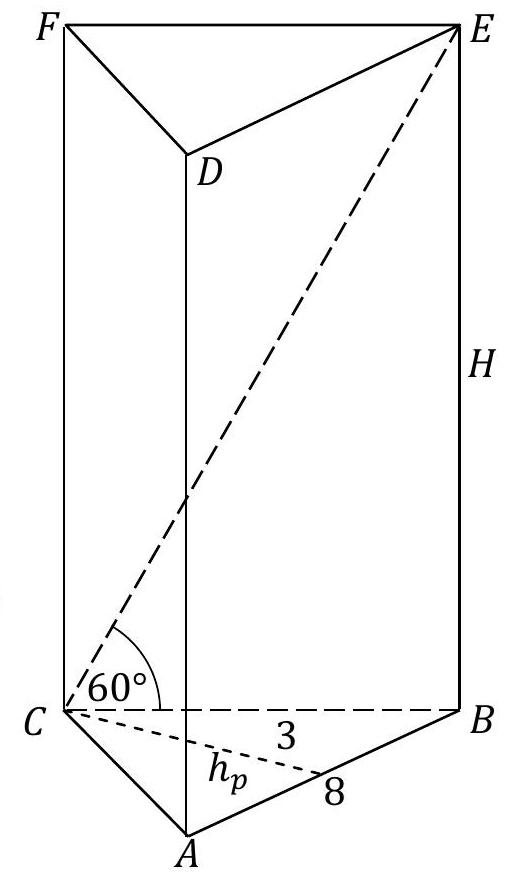
\includegraphics[max width=\textwidth]{2025_02_07_83b95a6405af75d2626bg-32}
\end{center}

Zatem $H=5 \sqrt{3}$.

Obliczamy pole powierzchni całkowitej graniastosłupa $A B C D E F$ :

$$
\begin{gathered}
P=P_{b}+2 P_{p}=2 \cdot H \cdot|B C|+|A B| \cdot H+2 \cdot \frac{1}{2} \cdot|A B| \cdot h_{p}=2 \cdot 5 \sqrt{3} \cdot 5+8 \cdot 5 \sqrt{3}+2 \cdot 12 \\
P=24+90 \sqrt{3}
\end{gathered}
$$

Obliczamy objętość $V$ graniastosłupa $A B C D E F$ :

$$
V=P_{p} \cdot H=12 \cdot 5 \sqrt{3}=60 \sqrt{3}
$$

\section*{Ocena prac osób ze stwierdzoną dyskalkulią}
Obowiązują Zasady oceniania stosowane przy sprawdzaniu prac zdających bez stwierdzonej dyskalkulii z dodatkowym uwzględnieniem:\\
a) ogólnych zasad oceniania zadań otwartych w przypadku arkuszy osób ze stwierdzoną dyskalkulią (punkty 1.-12.);\\
b) dodatkowych szczegółowych zasad oceniania zadań otwartych w przypadku arkuszy osób ze stwierdzoną dyskalkulią - egzamin maturalny z matematyki, poziom podstawowy, termin główny 2023.\\
I. Ogólne zasady oceniania zadań otwartych w przypadku arkuszy osób ze stwierdzoną dyskalkulią

\begin{enumerate}
  \item Nie należy traktować jako błędy merytoryczne pomyłek, wynikających z:
\end{enumerate}

\begin{itemize}
  \item błędnego przepisania
  \item przestawienia cyfr
  \item zapisania innej cyfry, ale o podobnym wyglądzie
  \item przestawienia położenia przecinka.
\end{itemize}

\begin{enumerate}
  \setcounter{enumi}{1}
  \item W przypadku błędów, wynikających ze zmiany znaku liczby, należy w każdym zadaniu oddzielnie przeanalizować, czy zdający opanował inne umiejętności, poza umiejętnościami rachunkowymi, oceniane w zadaniu. W przypadku opanowania badanych umiejętności zdający powinien otrzymać przynajmniej 1 punkt.
  \item We wszystkich zadaniach otwartych, w których wskazano poprawną metodę rozwiązania, części lub całości zadania, zdającemu należy przyznać przynajmniej 1 punkt, zgodnie z kryteriami do poszczególnych zadań.
  \item Jeśli zdający przedstawia nieprecyzyjne zapisy, na przykład pomija nawiasy lub zapisuje nawiasy w niewłaściwych miejscach, ale przeprowadza poprawne rozumowanie lub stosuje właściwą strategię, to może otrzymać przynajmniej 1 punkt za rozwiązanie zadania.
  \item W przypadku zadania wymagającego wyznaczenia pierwiastków trójmianu kwadratowego zdający może otrzymać 1 punkt, jeżeli przedstawi poprawną metodę wyznaczania pierwiastków trójmianu kwadratowego, przy podanych w treści zadania wartościach liczbowych.
  \item W przypadku zadania wymagającego rozwiązania nierówności kwadratowej zdający może otrzymać 1 punkt, jeżeli stosuje poprawny algorytm rozwiązywania nierówności kwadratowej, przy podanych w treści zadania wartościach liczbowych.
  \item W przypadku zadania wymagającego stosowania własności funkcji kwadratowej zdający może otrzymać 1 punkt za wykorzystanie konkretnych własności funkcji kwadratowej, istotnych przy poszukiwaniu rozwiązania.
  \item W przypadku zadania wymagającego zastosowania własności ciągów arytmetycznych lub geometrycznych zdający może otrzymać 1 punkt, jeżeli przedstawi wykorzystanie takiej własności ciągu, która umożliwia znalezienie rozwiązania zadania.
  \item W przypadku zadania wymagającego analizowania figur geometrycznych na płaszczyźnie kartezjańskiej zdający może otrzymać punkty, jeżeli przy poszukiwaniu rozwiązania przedstawi poprawne rozumowanie, wykorzystujące własności figur geometrycznych lub zapisze zależności, pozwalające rozwiązać zadanie.
  \item W przypadku zadania z rachunku prawdopodobieństwa zdający może otrzymać przynajmniej 1 punkt, jeśli przy wyznaczaniu liczby zdarzeń elementarnych sprzyjających rozważanemu zdarzeniu przyjmuje określoną regularność lub podaje prawidłową metodę wyznaczenia tej liczby zdarzeń elementarnych.
  \item W przypadku zadania z geometrii zdający może otrzymać przynajmniej 1 punkt, jeżeli podaje poprawną metodę wyznaczenia długości odcinka potrzebnej do znalezienia rozwiązania.
  \item W przypadku zadania wymagającego przeprowadzenia dowodu (z zakresu algebry lub geometrii), jeśli w przedstawionym rozwiązaniu zdający powoła się na własność, która wyznacza istotny postęp, prowadzący do przeprowadzenia dowodu, to może otrzymać 1 punkt.\\
II. Dodatkowe szczegółowe zasady oceniania zadań otwartych w przypadku arkuszy osób ze stwierdzoną dyskalkulią
\end{enumerate}

\section*{Zadanie 30.}
1 pkt - zastosowanie poprawnej metody obliczenia pierwiastków trójmianu kwadratowego $-x^{2}-2 x+3$, tzn. zastosowanie wzorów na pierwiastki trójmianu kwadratowego i obliczenie tych pierwiastków\\
ALBO

\begin{itemize}
  \item konsekwentne (do otrzymanego w wyniku popełnienia błędów o charakterze dyskalkulicznym ujemnego wyróżnika) narysowanie paraboli, ALBO
  \item poprawne rozwiązanie nierówności $x^{2}-2 x>0$ (tzn. stosuje się punkt 6 . ogólnych zasad oceniania), ALBO
  \item konsekwentne (do wyznaczonych przez siebie pierwiastków oraz rozpatrywanego trójmianu i nierówności) wyznaczenie zbioru rozwiązań nierówności.
\end{itemize}

\section*{Uwagi:}
\begin{enumerate}
  \item Jeżeli zdający, rozwiązując nierówność, pomyli porządek liczb na osi liczbowej i zapisze zbiór rozwiązań nierówności w postaci $(1,-3)$, to może otrzymać 2 punkty za całe rozwiązanie.
  \item Nie stosuje się uwag 2. i 3. z zasad oceniania arkusza standardowego.
\end{enumerate}

\section*{Zadanie 31.}
Stosuje się zasady oceniania arkusza standardowego.

\section*{Zadanie 32.}
Stosuje się zasady oceniania arkusza standardowego.

\section*{Zadanie 33.}
1 pkt - obliczenie długości $c_{1}$ przeciwprostokątnej trójkąta $T_{1}$ oraz wykorzystanie podobieństwa trójkątów i zapisanie związku między długościami przyprostokątnych trójkąta $T_{2}: c_{1}=13$ i $\frac{a_{2}}{b_{2}}=\frac{12}{5}$\\
ALBO

\begin{itemize}
  \item obliczenie długości $c_{1}$ przeciwprostokątnej trójkąta $T_{1}$ oraz zapisanie równania pozwalającego obliczyć długość jednej z przyprostokątnych trójkąta $T_{2}$, np.\\
$c_{1}=13$ i $\frac{13}{12}=\frac{26}{a_{2}}, c_{1}=13$ i $\frac{13}{5}=\frac{26}{b_{2}}$.
\end{itemize}

\section*{Zadanie 34.}
1 pkt - obliczenie współczynnika kierunkowego prostej $A C$ (lub zapisanie równania prostej $A C$ ): $\frac{3}{4}$.

\section*{Zadanie 35.}
1 pkt - zapisanie jedynie liczby 64 (należy traktować to jako wyznaczenie liczby wszystkich zdarzeń elementarnych).

\section*{Uwagi:}
\begin{enumerate}
  \item W ocenie rozwiązania tego zadania (dla zdających $z$ dyskalkulią) nie stosuje się uwagi ze standardowych zasad oceniania.
  \item Jeżeli zdający poprawnie wypisze/zaznaczy wszystkie zdarzenia elementarne sprzyjające zdarzeniu $A$, lecz popełni błąd w ich zliczeniu $(|A|=5)$ i konsekwentnie zapisze wynik $\frac{5}{64}$, to otrzymuje 2 punkty.
\end{enumerate}

\section*{Zadanie 36.}
Stosuje się zasady oceniania arkusza standardowego.


\end{document}